% Shared typesetting settings for the study booklets. Build from the project root.
\RequirePackage{array}[=2024-06-01]
% !TeX root = ../2/main.tex
\usepackage[a4paper,margin=25mm,headheight=16pt]{geometry}
\usepackage{amsmath,amssymb}
\usepackage{graphicx}
\usepackage{booktabs}
\usepackage{tabularx}
\usepackage{siunitx}
\usepackage{tikz}
\usepackage{circuitikz}
\usepackage[unicode,hidelinks]{hyperref}
\usepackage{xepersian}
% Only the regular B Nazanin file is installed; synthesize bold explicitly.
\settextfont[Path=C:/Windows/Fonts/,AutoFakeBold=2,AutoFakeSlant=0.2]{B-NAZANIN.TTF}
% B Nazanin lacks U+066A (Arabic percent), required by xepersian's digit setup.
% Arial covers the complete required digit/punctuation set; Persian prose remains B Nazanin.
\setdigitfont[Path=C:/Windows/Fonts/,BoldFont=arialbd.ttf,ItalicFont=ariali.ttf,BoldItalicFont=arialbi.ttf]{arial.ttf}
\setmathdigitfont[Path=C:/Windows/Fonts/,BoldFont=arialbd.ttf,ItalicFont=ariali.ttf,BoldItalicFont=arialbi.ttf]{arial.ttf}
\setlatintextfont{TeX Gyre Termes}
% B Nazanin does not contain the default itemize bullet and dash glyphs.
\renewcommand{\labelitemi}{\(\bullet\)}
\renewcommand{\labelitemii}{\(\circ\)}
\renewcommand{\labelitemiii}{\(\diamond\)}
\setlength{\parindent}{0pt}
\setlength{\parskip}{0.5em}
\linespread{1.25}
\newcommand{\exercise}[1]{\section*{تمرین #1}}
% !TeX root = ../2/main.tex
% Shared title page for every assignment.
% Change only \AssignmentNumber and \AssignmentDate in each main document.

\newcommand{\AssignmentNumber}[1]{\gdef\assignmentnumber{#1}}
\newcommand{\AssignmentDate}[1]{\gdef\assignmentdate{#1}}

\newcommand{\assignmentnumber}{---}
\newcommand{\assignmentdate}{---}

% Stable course metadata
\newcommand{\universityname}{دانشگاه صنعتی امیرکبیر}
\newcommand{\universityalias}{پلی‌تکنیک تهران}
\newcommand{\facultyname}{دانشکده مهندسی کامپیوتر}
\newcommand{\coursename}{طراحی مدارهای مجتمع پرتراکم پیشرفته}
\newcommand{\studentname}{محمد خلیلی اصل}
\newcommand{\instructorname}{دکتر مهدی صدیقی}

\newcommand{\MakeAssignmentCover}{%
  \begin{titlepage}
    \thispagestyle{empty}
    \centering
    \linespread{1}\selectfont

    \vspace*{0mm}
    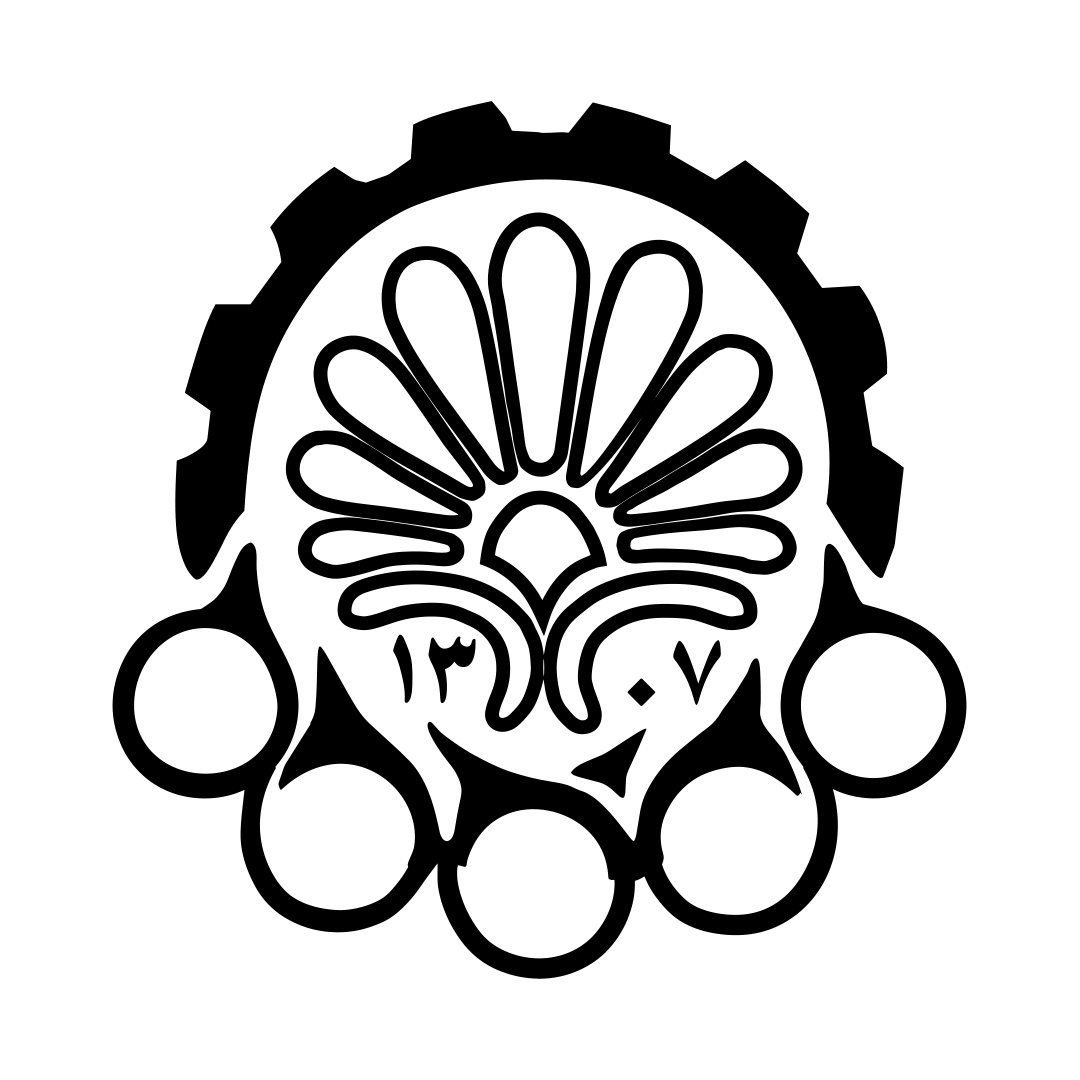
\includegraphics[width=44mm]{assets/aut-logo-black.png}\par
    \vspace{3mm}

    {\Large\bfseries \universityname\par}
    \vspace{1mm}
    {\large (\universityalias)\par}
    \vspace{1mm}
    {\large \facultyname\par}

    \vspace{8mm}
    {\Large\bfseries درس \coursename\par}

    \vspace{12mm}
    {\large عنوان\par}
    \vspace{2mm}
    {\LARGE\bfseries تمرین شماره \assignmentnumber\par}

    \vspace{10mm}
    {\large تهیه‌کننده\par}
    \vspace{2mm}
    {\Large\bfseries \studentname\par}

    \vspace{10mm}
    {\large استاد درس\par}
    \vspace{2mm}
    {\Large\bfseries \instructorname\par}

    \vspace{10mm}
    {\Large \assignmentdate\par}
    \vfill
  \end{titlepage}
  \setcounter{page}{1}%
}


\XeTeXgenerateactualtext=1
\newcommand{\secnum}[1]{\texorpdfstring{\mbox{\beginL#1\endL}}{#1}}
\newcommand{\code}[1]{\lr{\texttt{#1}}}
% Keep hierarchical counters in logical left-to-right order with localized digits.
\renewcommand{\thesection}{\texorpdfstring{\secnum{\arabic{chapter}.\arabic{section}}}{\arabic{chapter}.\arabic{section}}}
\renewcommand{\thesubsection}{\texorpdfstring{\secnum{\arabic{chapter}.\arabic{section}.\arabic{subsection}}}{\arabic{chapter}.\arabic{section}.\arabic{subsection}}}
\renewcommand{\thesubsubsection}{\texorpdfstring{\secnum{\arabic{chapter}.\arabic{section}.\arabic{subsection}.\arabic{subsubsection}}}{\arabic{chapter}.\arabic{section}.\arabic{subsection}.\arabic{subsubsection}}}
\counterwithin*{equation}{section}
\renewcommand{\theHequation}{\arabic{chapter}.\arabic{section}.\arabic{equation}}
\renewcommand{\theequation}{\texorpdfstring{\secnum{\theHequation}}{\theHequation}}
\renewcommand{\thefigure}{\texorpdfstring{\secnum{\arabic{chapter}.\arabic{figure}}}{\arabic{chapter}.\arabic{figure}}}
\renewcommand{\thetable}{\texorpdfstring{\secnum{\arabic{chapter}.\arabic{table}}}{\arabic{chapter}.\arabic{table}}}
\makeatletter
\renewcommand{\@pnumwidth}{2.5em}
\renewcommand{\@tocrmarg}{3.5em}
\makeatother
% Preserve the reviewed fragments while nesting their teaching units under the source section.
\newcommand{\BookletSubsections}[1]{%
  \begingroup
  \let\section\subsection
  \let\subsection\subsubsection
  \input{#1}%
  \endgroup
}
\setlength{\emergencystretch}{3em}
\widowpenalty=10000
\clubpenalty=10000
\setcounter{secnumdepth}{3}
\AtBeginDocument{\DeclareSIPrefix{\micro}{\text{\lr{µ}}}{-6}}
\patchcmd{\MakeAssignmentCover}{تمرین شماره \assignmentnumber}{\assignmentnumber}{}{\errmessage{Cover title replacement failed}}
% Shared bibliographic text. Coverage notes remain in each booklet.
\newcommand{\WesteReference}{%
\begin{latin}
Neil H. E. Weste and David Money Harris,
\textit{CMOS VLSI Design: A Circuits and Systems Perspective},
Fourth Edition, Addison-Wesley (Pearson Education), 2011.
\end{latin}%
}


% The complete edition continues textbook chapter 2 across all three booklets.
\newif\ifCompleteNotes
\newcommand{\NotesTopic}[2]{%
  \ifCompleteNotes\hyperref[#1]{#2}\else#2\fi
}
% Topic reviews are nested under their host section in the comprehensive notes.
\newcommand{\BookletReview}[1]{%
  \ifCompleteNotes
    \begingroup
    \let\chapter\subsection
    \let\section\subsubsection
    \let\BookletAddContentsLine\addcontentsline
    \renewcommand{\addcontentsline}[3]{%
      \ifstrequal{##2}{chapter}
        {\BookletAddContentsLine{##1}{subsection}{##3}}
        {\ifstrequal{##2}{section}
          {\BookletAddContentsLine{##1}{subsubsection}{##3}}
          {\BookletAddContentsLine{##1}{##2}{##3}}}%
    }%
    \input{#1}%
    \endgroup
  \else
    \input{#1}%
  \fi
}
